\section{Methodlogy}


In this section, using tradeflow data for the year 2022, along with specifications from the IHS dataset, we will perform data analysis.

Tradetable data is available in the \texttt{tradetable13bx} dataset. For each segments there is \texttt{tradetable13bx} and thereforre we will have to perform the analysis for each segment separately.

The steps involved in the analysis are as follows:

\newpage

\subsubsection{1. Getting distinct IMO numbers from tradetable13bx}

Distinct IMO numbers can be obtained from the \texttt{tradetable13bx} dataset by querying the \texttt{imo} column.
This will give us a list of all ships that are present in the dataset.

\begin{lstlisting}[language=python, caption=SQL Query to get distinct IMO]
    vlccImoQuery = spark.sql(f"""
        SELECT DISTINCT(imo) FROM vlcc.tradetable13bx
    """)
\end{lstlisting}

\subsubsection{2. Getting necessary information for each IMO number from IHS and tradetable13bx}
For each IMO number obtained in the previous step,
query the IHS dataset or join it with \texttt{tradetable13bx} to gather relevant information about each ship, such as its specifications, fuel type, engine types, etc.



\begin{lstlisting}[language=python, caption=SQL Query to get relevent data from \texttt{ihs} and \texttt{tradetable13bx}]
            shipTrade = spark.sql(f"""
                SELECT 
                    st.Imo,
                    st.AverageSpeedAB,
                    st.LoadAtB,
                    st.UnloadAtB,
                    st.ShipName,
                    st.FromPortA,
                    st.ToPortB,
                    st.DepartA,
                    st.ArriveB,
                    st.HoursAtAMax,
                    st.HoursAtBMax,
                    st.ArriveDraughtB,
                    st.DraughtChangeB,
                    st.DistanceAB,
                    st.HoursAB,
                    st.EstimatedDischargePct,
                    ihs.deadweight,
                    ihs.draught as maxDraught,
                    sp.ballast_threshold_pct as ballastThreshold,
                    ABS(round((st.ArriveDraughtB * 100) /ihs.draught)) as draughtPercentage,
                    ABS(round(ihs.deadweight*st.EstimateddischargePct/100,0)) as cargoEst,
                    ABS(round((ihs.deadweight*st.ArriveDraughtB)/ihs.draught)) as cargoEst2,
                        CASE 
                            WHEN 
                                st.ArriveDraughtB >= (ihs.draught * sp.ballast_threshold_pct / 100.0) 
                            THEN 'laden'
                            ELSE 'ballast'
                        END AS loadCond
                FROM vlcc.tradetable13bx as st
                JOIN ihs_ship_data_ ihs on ihs.lrimoshipno = st.Imo
                JOIN ( 
                        select * from parameters.segment_parameters  where segment = '{segment}'
                    ) sp on true
                WHERE st.Imo = {imo} AND st.DepartA  between '{startDate}' AND '{endDate}' AND st.ArriveDraughtB IS NOT null
                ORDER BY st.DepartA
                      
                """)
          \end{lstlisting}

Here, we have estimated cargo based on draught noted on ports and maximum draught from IHS dataset.
Also to deptermine whether the tradeflow is laden or ballast, we have used ballast threshold percentage from segment parameters.

Threshold for each sections are as showin in figure \ref{segment_parameters}:

\begin{figure}[h]
    \centering
    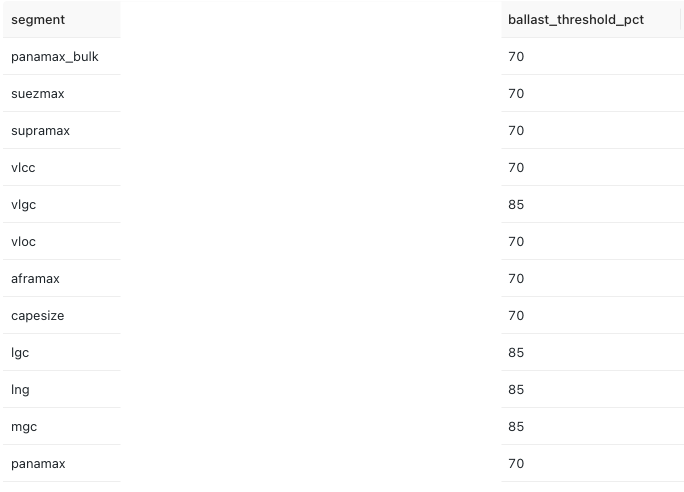
\includegraphics[width=1\textwidth]{images/segment_parameters.png}
    \caption{Ballast Threshold Percentage}
    \label{segment_parameters}
\end{figure}

\texttt{shipTrade} obtained  is converted into pandas dataframe and then processed further.

\begin{lstlisting}[language=python, caption=shipTrade pandas dataframe]
    shipTradePandas = shipTrade.toPandas()
\end{lstlisting}

Further trade is divided into dataframes for laden and ballast tradeflows.

\begin{lstlisting}[language=python, caption=laden and ballast tradeflows]
    ladenTrade = shipTradePandas[shipTradePandas["loadCond"] == 'laden']
    ballastTrade = shipTradePandas[shipTradePandas["loadCond"] == 'ballast']
\end{lstlisting}

Then we extract information like distance, time and average speed for both ballast and laden tradeflows.

\begin{lstlisting}[language=python, caption={Determing distance, time and average speed}]
    totalLadenDistance = ladenTrade["DistanceAB"].sum()
    totalBallastDistance = ballastTrade["DistanceAB"].sum()
    totalDistance = shipTradePandas["DistanceAB"].sum()

    totalLadenHours = ladenTrade["HoursAB"].sum()
    totalBallastHours = ballastTrade["HoursAB"].sum()
    totalHours = shipTradePandas["HoursAB"].sum()

    ladenAvgSpeed = ladenTrade["AverageSpeedAB"].mean()
    ladenAvgSpeed2 = totalLadenDistance / totalLadenHours
    
    ballastAvgSpeed = ballastTrade["AverageSpeedAB"].mean()
    ballastAvgSpeed2 = totalBallastDistance / totalBallastHours
  
    cargo2 = ladenTrade["cargoEst2"].sum()


\end{lstlisting}

\subsubsection{3. Cleaning data}

Data cleaning involves handling missing values, removing duplicates, standardizing units, and correcting any inconsistencies in the dataset.

When determining average speed, speed determined from AIS data might be missing for some tradeflows.
Also sometimes, it was noticed that averge speed was very high for some tradeflows.
In such cases, we can use the distance and time values to calculate average speed.


\begin{lstlisting}[language=python, caption=Handling missing speed]
    if (ladenAvgSpeed < 0 or ladenAvgSpeed > ladenAvgSpeed2):
      ladenAvgSpeed = ladenAvgSpeed2
    if (ladenAvgSpeed > 15):
      ladenAvgSpeed = 15
\end{lstlisting}

Sometimes for certain trades average distance was missing, this trades were excluded.

\subsubsection{4. Calculating emissions for laden and ballast tradeflows.}

Using the information extracted in the previous steps, emissions is calculated using AFC emission calculator API.

For this \texttt{getEmission} function is used which takes IMO number, cargo amount, distance, load condition and estimated speed as input and returns emissions.
As showin in Listing \ref{getEmission}.

\begin{lstlisting}[language=python, caption=Handling missing speed, label=getEmission]
    def getEmission(imo, cargo_amt, distance_nm, load_cond, est_speed):
        token = get_token()
        
        data_string = f"imo={imo}&cargo_amt={cargo_amt}&distance_nm={distance_nm}&duration_h={duration_h}&load_cond={load_cond}"
        
        url = url_start + data_string

        payload={}
        headers = {
        'Ocp-Apim-Subscription-Key': 'xxxxxxxxxxx',
        'Authorization': 'Bearer ' + token
        }

        response = requests.request("GET", url, headers=headers, data=payload)
        time.sleep(0.04)
        try:
            response_dict = json.loads(response.text)
            return response_dict
        except BaseException as e:
            print("error", e)
            print("error in url", url)
            return None
\end{lstlisting}


\subsubsection{Calculating CII, CII required, and CII reference.}

Carbon Intensity Indicator (CII) is calculated as the ratio of emissions (CO\textsubscript{2}) to transport work (distance traveled $\times$ cargo amount). CII required is based on regulatory standards, while CII reference can be derived from historical data or benchmarks. Calculate these indicators for each tradeflow using the emission data and transport work values.

\subsubsection{Calculating CII grade.}

Based on the calculated CII and CII required, determine the CII grade for each tradeflow, indicating its compliance with emissions regulations. This can be done using predefined thresholds or standards to categorize tradeflows into different CII grades.

